
\documentclass[12pt,a4paper]{article}

\usepackage[a4paper,margin=1in]{geometry}
\usepackage{graphicx}
\usepackage{booktabs}
\usepackage{amsmath,amssymb}
\usepackage{float}
\usepackage{hyperref}
\usepackage{xcolor}
\usepackage{listings}
\usepackage{enumitem}
\usepackage{fancyhdr}
\usepackage{longtable}

\hypersetup{colorlinks=true,linkcolor=blue,urlcolor=blue}

\pagestyle{fancy}
\fancyhf{}
\lhead{ICS1512}
\rhead{Machine Learning Algorithms Laboratory}
\cfoot{\thepage}

\lstset{
language=Python,
basicstyle=\ttfamily\small,
numbers=left,
frame=single,
breaklines=true,
showstringspaces=false
}

\begin{document}

\begin{tabular}{|p{4cm}|p{11cm}|}
\hline
Experiment No. & 2 \\ \hline
Experiment Title & Email Spam/Ham Classification using Naive Bayes and KNN\footnotemark \\ \hline
Student Name & Sanjay S \\ \hline
Register Number & 3122247001056 \\ \hline
Faculty & Dr. Poreddy Ajay Kumar Reddy \\ \hline
Submission Date & 03/08/2026 \\ \hline
\end{tabular}
\footnotetext{\textbf{GitHub Repository: }\url{https://github.com/sanjay-6727/Introdution-to-Machine-Learning-}}

\section{Objective}
Build spam classifiers with Naive Bayes and KNN, compare the Gaussian, Multinomial and Bernoulli
variants against each other, see how accuracy moves with $k$, pit KDTree against BallTree, tune KNN
with both GridSearchCV and RandomizedSearchCV, and keep an eye on speed the whole way through, not just
accuracy.

\section{Problem Statement}
Given Spambase, 4601 emails described by 57 numeric features (word and character frequencies plus
capital-letter run stats), predict spam or ham, and actually compare how differently Naive Bayes and
KNN behave on the exact same data, speed included.

\section{Dataset Description}
\begin{longtable}{|p{6cm}|p{8cm}|}
\hline
Dataset Name & Spambase \\ \hline
Dataset Source & Kaggle, somesh24/spambase (originally UCI ML Repository) \\ \hline
Number of Samples & 4601 \\ \hline
Number of Features & 57 \\ \hline
Number of Classes & 2 (spam = 1, ham = 0) \\ \hline
Missing Values & none \\ \hline
Train-Test Split & 80/20, stratified, plus 5 fold cross validation \\ \hline
\end{longtable}

\section{Exploratory Data Analysis}
\begin{itemize}
\item Class distribution: 2788 ham vs 1813 spam, so mildly imbalanced but nothing extreme.
\item Correlation and feature distribution: heavily right skewed word frequencies, computed for the
ten features most correlated with the label.
\item No missing values to deal with here, which was a nice change of pace.
\end{itemize}

\begin{figure}[H]
\centering
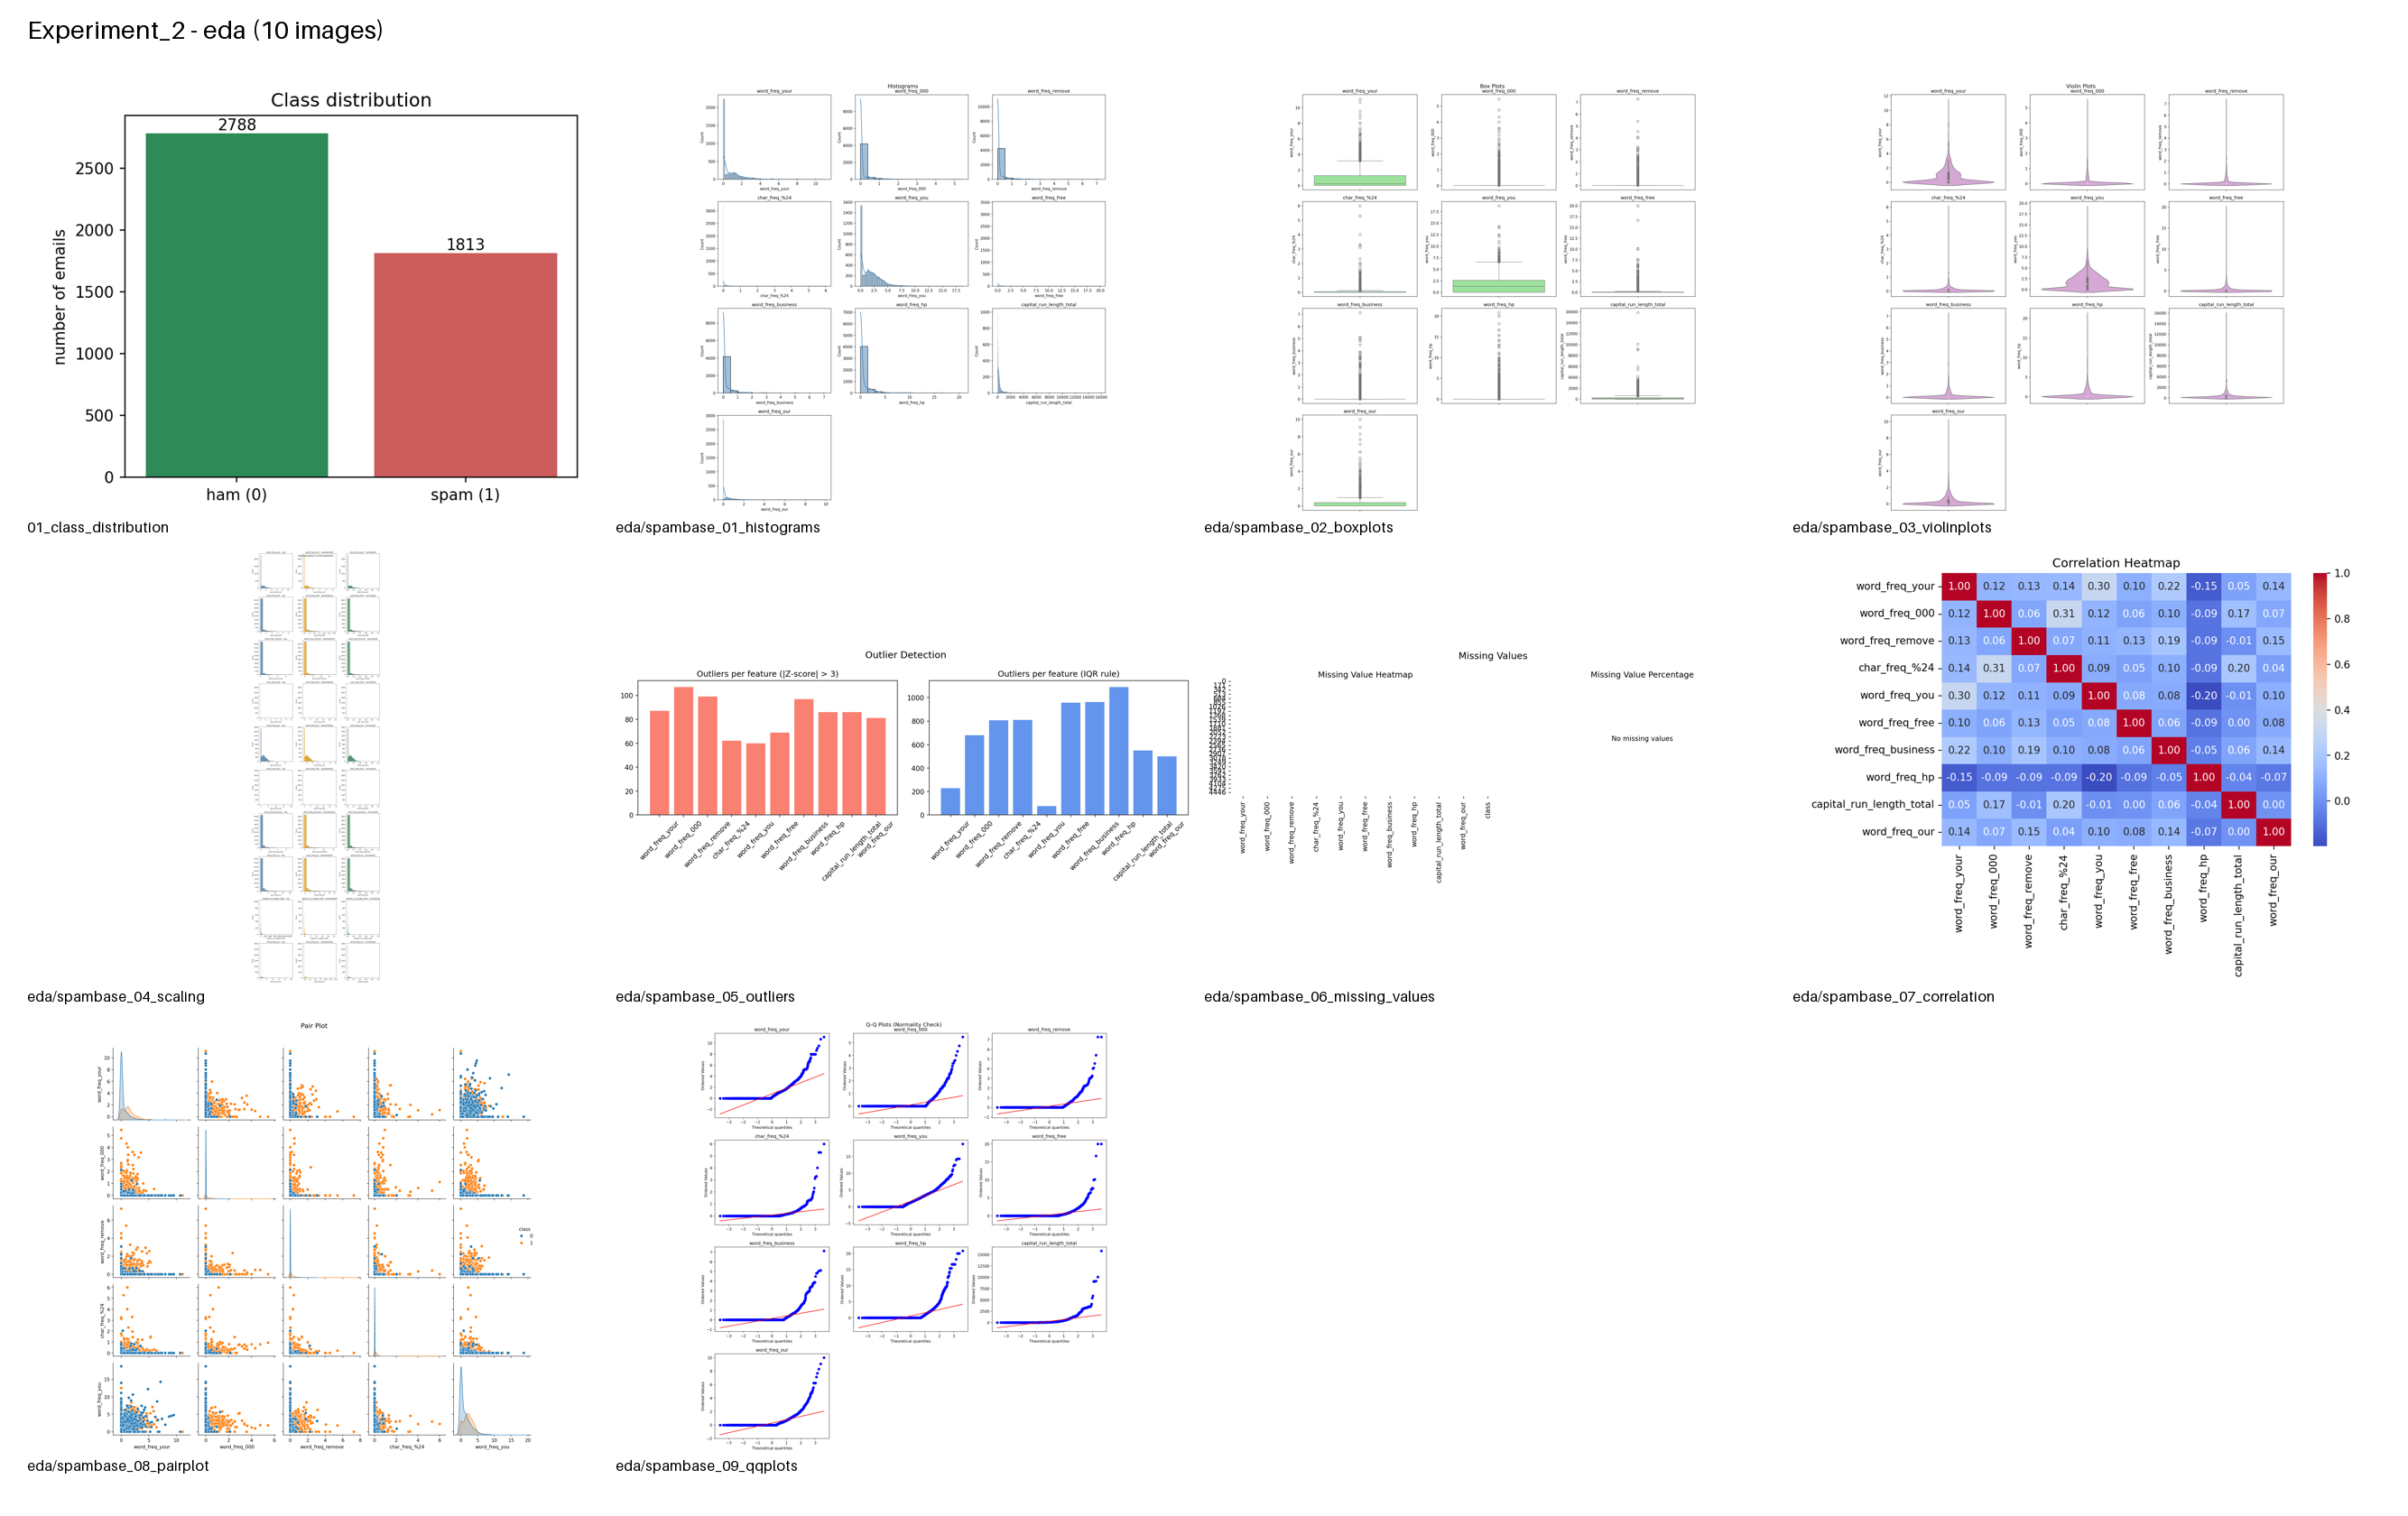
\includegraphics[width=0.95\linewidth]{outputs/Experiment_2_eda_combined.png}
\caption{Class distribution, full correlation heatmap, and histogram, box plot, violin, scaling,
outlier, pair plot and Q-Q panels for the ten most predictive features.}
\end{figure}

\textbf{Inference:}

word\_freq\_your, word\_freq\_000, word\_freq\_remove and the exclamation mark frequency come out as
the strongest correlates of spam, which lines up pretty well with how spam actually reads. Most
features spike hard at zero with a long thin tail, makes sense given any one email only touches a
handful of the tracked words. Even the pair plot on its own shows some real separation between spam
and ham, which is a good early sign a fairly simple classifier should do okay here.

\section{Data Preprocessing}
\begin{itemize}
\item No missing values, no encoding needed, all 57 features come in numeric already.
\item Gaussian NB and KNN trained on StandardScaler output. Multinomial and Bernoulli NB trained on
the raw counts instead, since both expect non-negative input and scaling would wreck that.
\item 80/20 stratified split, with 5 fold cross validation used throughout tuning.
\end{itemize}

\begin{lstlisting}[caption={Naive Bayes variants: Gaussian on scaled data, Multinomial/Bernoulli on raw counts}]
gnb = GaussianNB().fit(X_train_scaled, y_train)
mnb = MultinomialNB().fit(X_train_raw, y_train)
bnb = BernoulliNB().fit(X_train_raw, y_train)

grid = GridSearchCV(KNeighborsClassifier(), param_grid,
                     cv=5, scoring="accuracy", n_jobs=-1)
grid.fit(X_train_scaled, y_train)
print(grid.best_params_, grid.best_score_)
\end{lstlisting}

\section{Machine Learning Algorithm}

\textbf{Naive Bayes} applies Bayes' theorem with a conditional independence assumption:
$P(C \mid X) = \frac{P(X \mid C)P(C)}{P(X)}$. Gaussian NB assumes normal features, Multinomial models
counts, and Bernoulli treats everything as presence or absence. All three train fast, but that
independence assumption does cost you accuracy once features start correlating with each other.

\textbf{K-Nearest Neighbors} just stores the training set and votes among the $k$ closest points when
it actually needs to predict something. No real assumption about the boundary shape, which is nice, but
every single prediction means a distance search, so it ends up being the pricier of the two at
inference time.

\section{Experimental Setup}
\begin{tabular}{ll}
\toprule
Python Version & 3.11.9 \\
Scikit-Learn Version & 1.7.2 \\
IDE & Anaconda Navigator / VS Code \\
Operating System & Windows 11 \\
Hardware & \\
\bottomrule
\end{tabular}

\section{Hyperparameter Selection}
\begin{tabular}{p{4.2cm}p{9.5cm}}
\toprule
Parameter & Value\\
\midrule
KNN k values tried & 1, 3, 5, 7, 9, 11 \\
GridSearchCV grid & n\_neighbors in \{1,3,5,7,9,11,15,21\}, weights, metric, algorithm \\
GridSearchCV best & k=11, manhattan, distance, kd\_tree, CV accuracy 0.9228 \\
RandomizedSearchCV best & k=9, manhattan, distance, kd\_tree, CV accuracy 0.9212 \\
\bottomrule
\end{tabular}

\section{Results}

\textbf{Naive Bayes comparison}

\begin{tabular}{lccc}
\toprule
Metric & Gaussian & Multinomial & Bernoulli \\
\midrule
Accuracy & 0.8328 & 0.7763 & 0.8762 \\
Precision & 0.7146 & 0.7199 & 0.8716 \\
Recall & 0.9587 & 0.7080 & 0.8044 \\
F1 & 0.8188 & 0.7139 & 0.8367 \\
ROC-AUC & 0.9376 & 0.8248 & 0.9496 \\
\bottomrule
\end{tabular}

\vspace{0.3cm}
\textbf{KNN across k}

\begin{tabular}{lcccc}
\toprule
k & Accuracy & Precision & Recall & F1 \\
\midrule
1 & 0.8990 & 0.8792 & 0.8623 & 0.8707 \\
5 & 0.9077 & 0.8861 & 0.8788 & 0.8824 \\
9 & 0.9088 & 0.8930 & 0.8733 & 0.8830 \\
11 & 0.9099 & 0.9000 & 0.8678 & 0.8836 \\
\bottomrule
\end{tabular}

\vspace{0.3cm}
\textbf{KDTree vs BallTree (k=11)}

\begin{tabular}{lcc}
\toprule
Metric & KDTree & BallTree \\
\midrule
Accuracy & 0.9099 & 0.9099 \\
Training Time (s) & 0.0266 & 0.0180 \\
Prediction Time (s) & 0.2015 & 0.1827 \\
\bottomrule
\end{tabular}

\vspace{0.3cm}
\textbf{Measured training / prediction time}

\begin{tabular}{lcc}
\toprule
Algorithm & Train (s) & Predict (s) \\
\midrule
Gaussian NB & 0.00398 & 0.00079 \\
Bernoulli NB & 0.00548 & 0.00172 \\
Best KNN (tuned) & 0.02411 & 0.19402 \\
\bottomrule
\end{tabular}

\section{Result Visualization}

\begin{figure}[H]
\centering
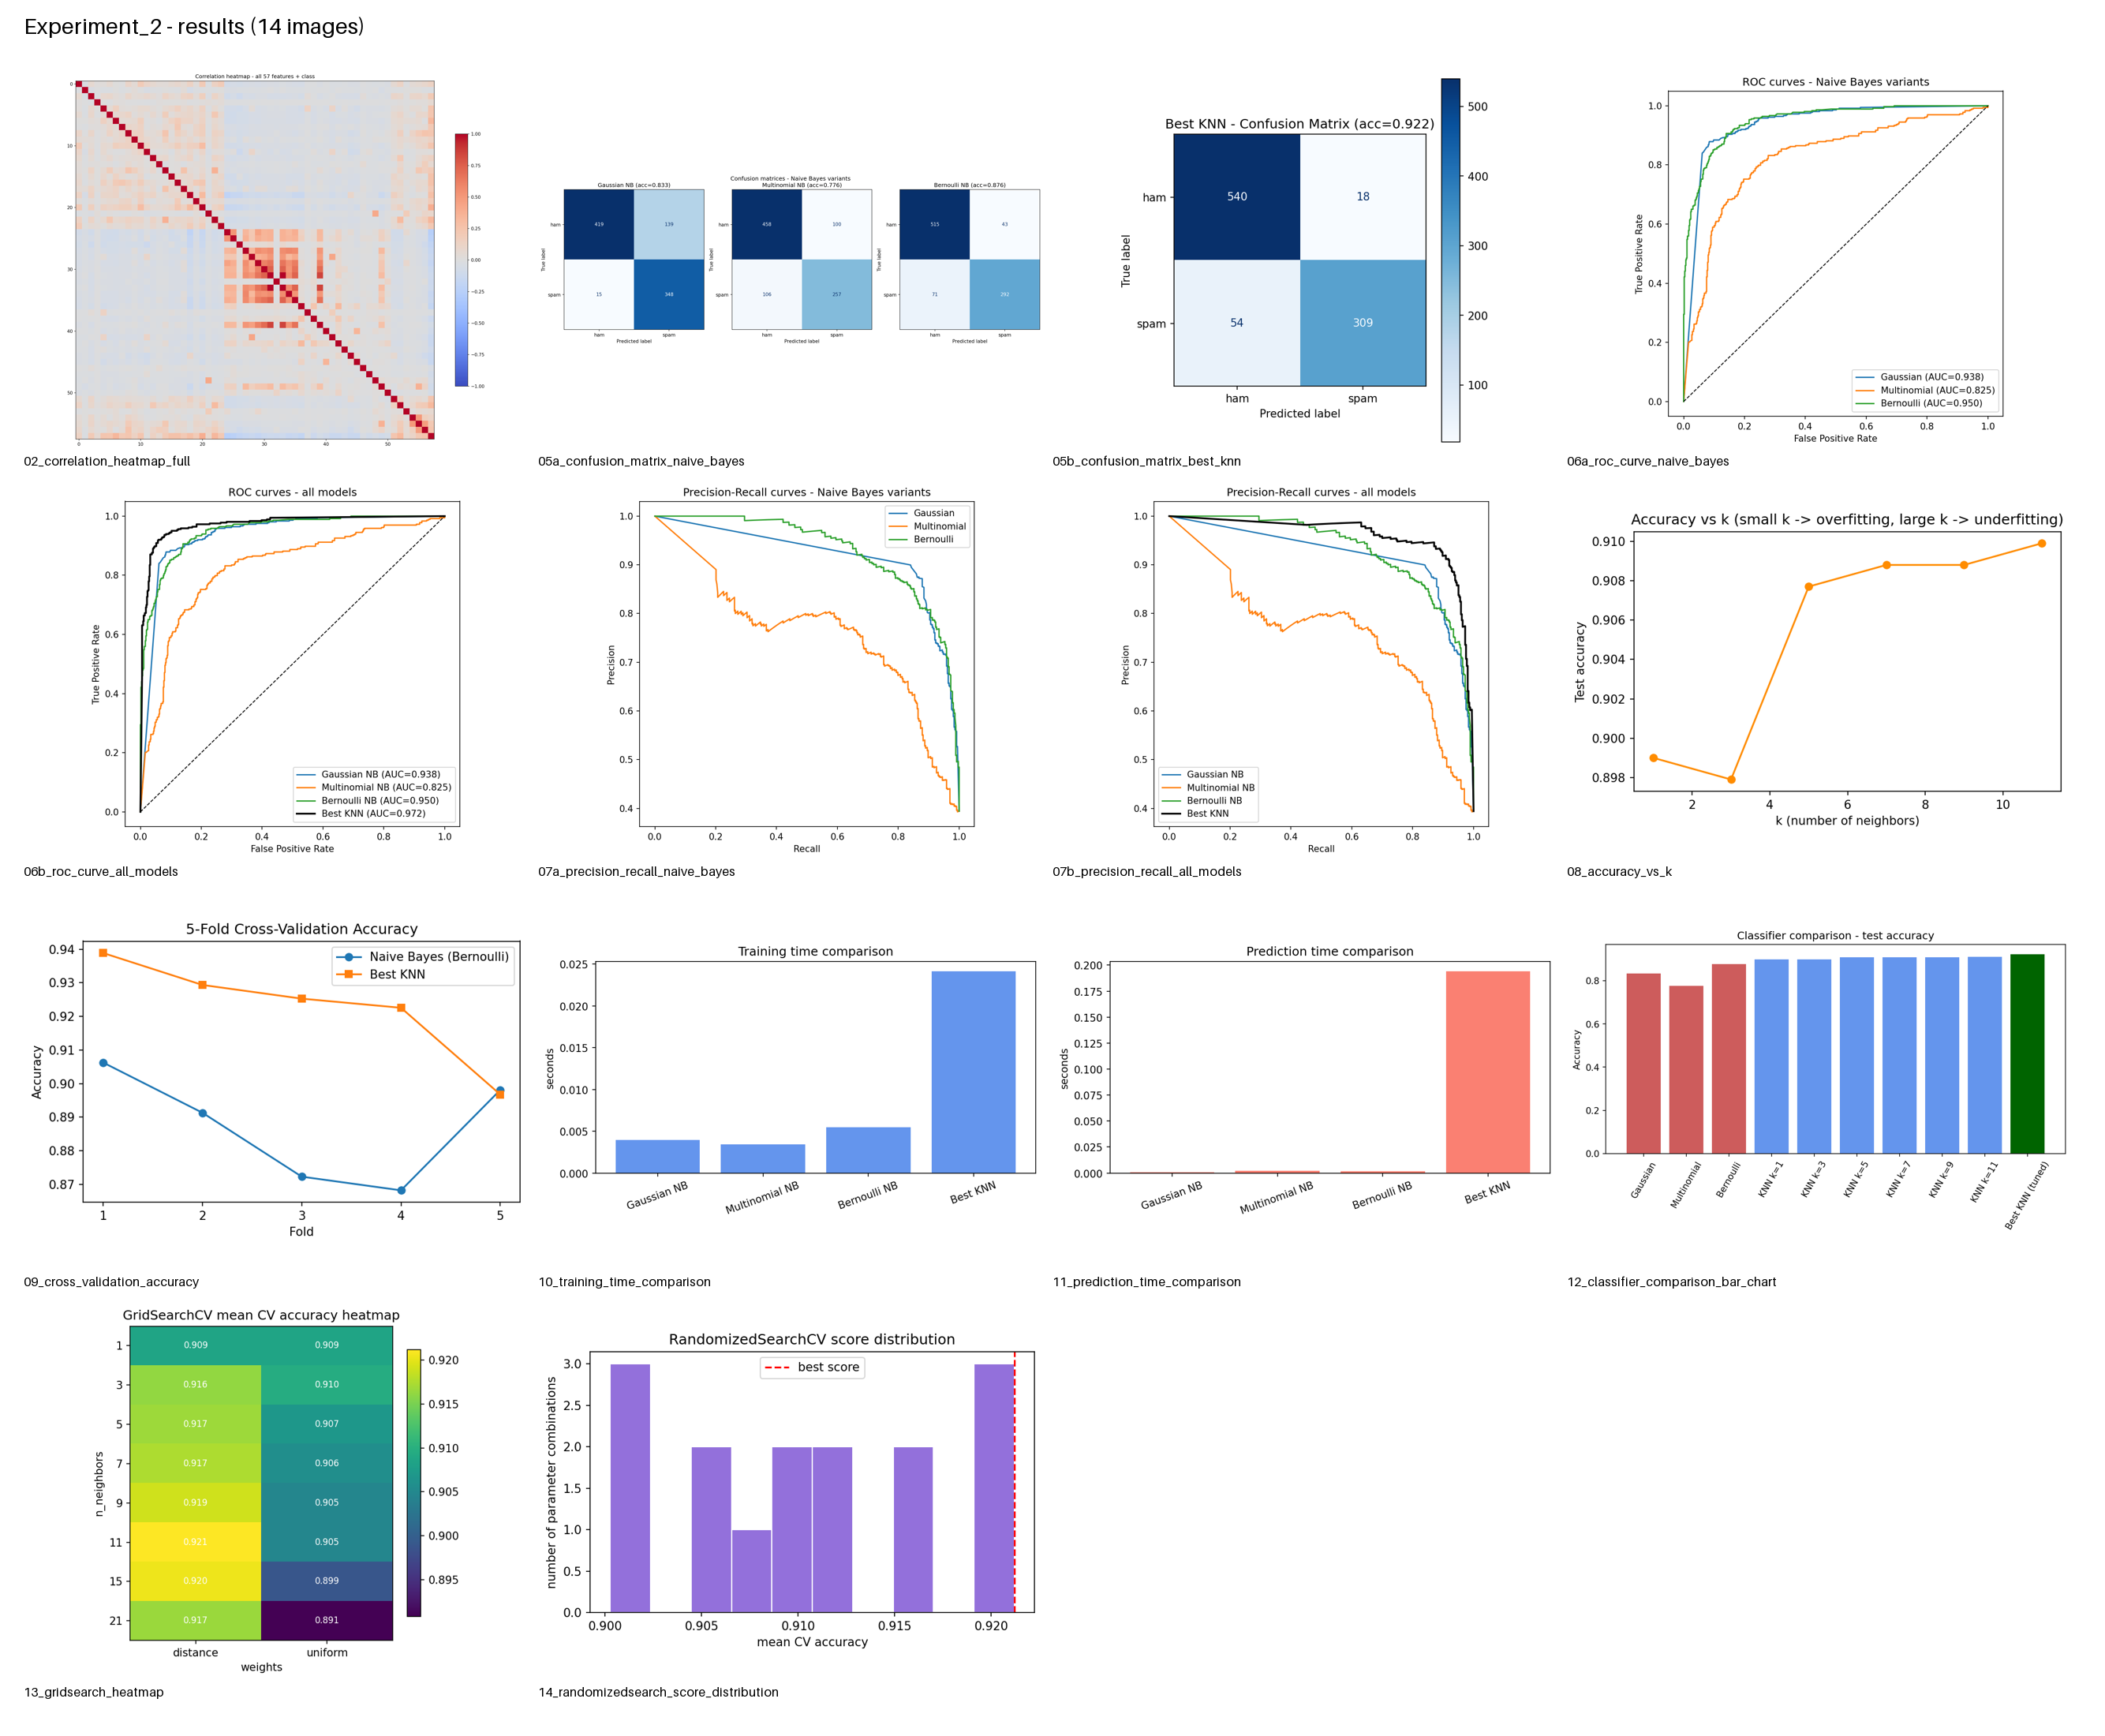
\includegraphics[width=0.95\linewidth]{outputs/Experiment_2_results_combined.png}
\caption{Confusion matrices, ROC and precision-recall curves, accuracy vs k, cross validation
accuracy, timing bars, classifier comparison, GridSearchCV heatmap and RandomizedSearchCV score
distribution.}
\end{figure}

\textbf{Inference:}

Bernoulli NB takes the three way comparison pretty clearly, best accuracy, precision and ROC-AUC of
the bunch, which fits with Spambase behaving more like presence/absence data than raw counts. Gaussian
NB does have the best recall though, it just pays for that with a lot of false positives along the
way. The accuracy vs k curve climbs up to around k=9 or 11 and then flattens out, small k is basically
overfitting to noisy neighbors while a much larger k would start underfitting. GridSearchCV and
RandomizedSearchCV landed on almost identical accuracy even though the randomized version only checked
a fraction of the combinations and finished roughly eight times faster, which says a lot about when the
cheaper search is worth using. KDTree and BallTree came out with identical accuracy, as they should,
since only their search speed differs, not what they actually return. And the timing bars really do
say it all here, Naive Bayes runs in milliseconds no matter what, while KNN's prediction time is easily
the most expensive thing on the whole chart.

\section{Discussion}
Naive Bayes' independence assumption clearly costs it accuracy next to tuned KNN, 0.8872 versus 0.9226
average CV accuracy, but it wins easily on speed, and that gap would only get wider with more data.
Bernoulli NB beating the other two variants makes sense once you accept Spambase is closer to a
presence/absence signal than a true count signal. KNN's prediction time already looks a bit much at
only 4601 rows, so scaling this further would really need an approximate search method rather than
brute KDTree or BallTree lookups.

\section{Conclusion}
Tuned KNN wins on raw accuracy against every Naive Bayes variant, but Naive Bayes is dramatically
cheaper to run. For something like a high volume mail filter, that tradeoff could easily flip the
decision back toward Naive Bayes. GridSearchCV and RandomizedSearchCV landing so close together also
gives some confidence that k=11 with manhattan distance and distance weighting is a genuinely solid
setting here, not just something the search got lucky on.

\section{Learning Outcomes}
\begin{itemize}
\item Saw firsthand how the independence assumption in Naive Bayes trades away accuracy in exchange
for a big speed win.
\item Got why KNN needs scaled features, and that its real bottleneck is prediction time, not training.
\item Ran GridSearchCV and RandomizedSearchCV side by side and watched the randomized version land
almost the same answer for a fraction of the cost.
\item Learned that KDTree and BallTree change search speed only, never the actual predictions.
\end{itemize}

\section{References}
\begin{enumerate}
\item Stephen Marsland, ``Machine Learning - An Algorithmic Perspective'', 2nd Edition, Chapman and
Hall/CRC Machine Learning and Pattern Recognition Series, 2015.
\item Ethem Alpaydin, ``Introduction to Machine Learning'', 3rd Edition, The MIT Press, 2014.
\end{enumerate}

\end{document}
